\documentclass[a4paper]{report}
\usepackage[utf8]{inputenc}
\usepackage[portuguese]{babel}
\usepackage{hyperref}
\usepackage{a4wide}
\hypersetup{pdftitle={TP3:  Protocolo IP},
    pdfauthor={João Teixeira, José Ferreira, Miguel Solino},
    colorlinks=true,
    urlcolor=blue,
    linkcolor=black}
\usepackage{subcaption}
\usepackage[cache=false]{minted}
\usepackage{listings}
\usepackage{booktabs}
\usepackage{multirow}
\usepackage{appendix}
\usepackage{tikz}
\usepackage{authblk}
\usepackage{bashful}
\usepackage{verbatim}
\usepackage{amsmath}
\usetikzlibrary{positioning,automata,decorations.markings}
\AfterEndEnvironment{figure}{\noindent\ignorespaces}

\begin{document}

\title{TP4:\\ 
    \large Grupo Nº 7}
\author{João Teixeira (A85504) \and José Ferreira (A83683) \and Miguel Solino (A86435)}

\date{\today}

\begin{center}
    \begin{minipage}{0.75\linewidth}
        \centering
        
\includegraphics[width=0.4\textwidth]{images/eng.jpeg}\par\vspace{1cm}
        \vspace{1cm}
        \href{https://www.uminho.pt/PT}
        {\color{black}{\scshape\LARGE Universidade do Minho}} \par
        \vspace{1cm}
        \href{https://www.di.uminho.pt/}
        {\color{black}{\scshape\Large Departamento de Informática}} \par
        \maketitle
    \end{minipage}
\end{center}

\tableofcontents
\chapter{3. Acesso Rádio}

\begin{figure}[H]
    \centering 
    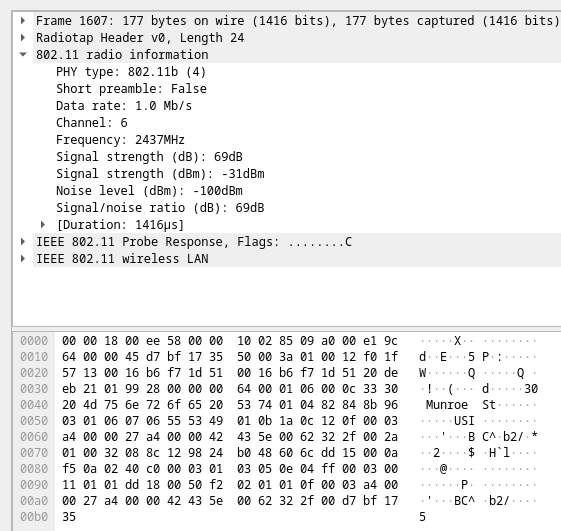
\includegraphics[width=\textwidth]{images/trama1607.png}  
    \caption{Trama 1607}
    \label{fig:trama1607}
\end{figure}

\section{Exercício 1}
\textbf{Identifique em que frequência do espectro está a operar a rede sem fios,
e o canal que corresponde a essa frequência.}\\
Observando a figura \ref{fig:trama1607}, a frequência do espectro que está a
operar a rede sem fios é 2437MHz, correspondente ao canal 6.

\section{Exercício 2}
\textbf{Identifique a versão da norma IEEE 802.11 que está a ser usada.}\\
Reparando no campo PHY type na figura \ref{fig:trama1607}, a versão da norma
IEEE é a 802.11b.

\section{Exercício 3}
\textbf{Qual o débito a que foi enviada a trama escolhida? Será que esse débito
corresponde ao débito máximo a que a interface Wi-Fi pode operar?
Justifique.}

\begin{figure}[H]
    \centering 
    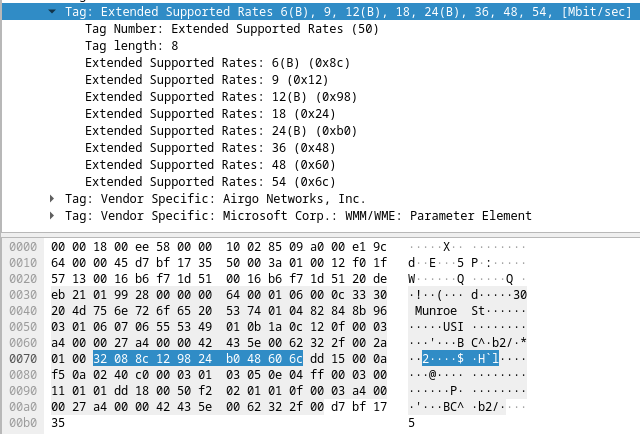
\includegraphics[width=\textwidth]{images/maxDataRateEx3.png}  
    \caption{Extended Suported Rates da trama 1607}
    \label{fig:maxDataRateEx3}
\end{figure}
Como é visto nas figuras \ref{fig:trama1607} e \ref{fig:maxDataRateEx3}, verificamos
que o débito usado para o envio é de 1.0MB/s e o débito máximo teórico é 54MB/s.
Logo o débito a que foi enviado não corresponde ao máximo da interface Wi-Fi.

\chapter{4. Scanning}
\section{Exercício 4}
\textbf{Quais são os SSIDs dos dois APs que estão a emitir a maioria das tramas
de beacon?}

\begin{figure}[H]
    \centering 
    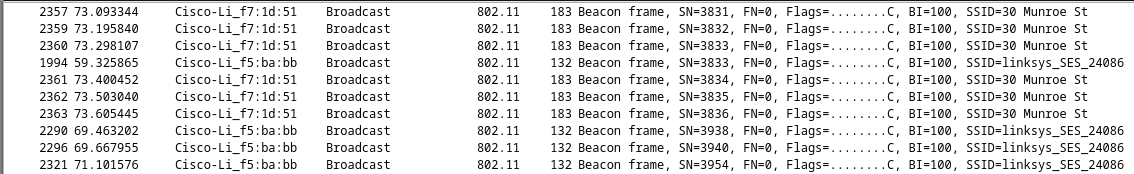
\includegraphics[width=\textwidth]{images/SSIDsEx4.png}  
    \caption{SSIDs mais frequentes}
    \label{fig:SSIDsEx4}
\end{figure}
Como é mostrado na figura \ref{fig:SSIDsEx4}, os dois APs que estão a emitir a
maioria das tramas são 30 Munroe St e linksys\_SES\_24086.

\section{Exercício 5}
\textbf{Qual o intervalo de tempo entre a transmissão de tramas beacon para o AP
linksys\_ses\_24086? E do AP 30 Munroe St? (Pista: o intervalo está contido na
própria trama). Na prática, a periodicidade de tramas beacon é verificada?
Tente explicar porquê.}

\begin{figure}[H]
    \centering 
    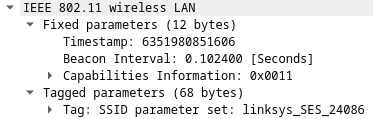
\includegraphics[width=\textwidth]{images/tramaLinkEx5.png}  
    \caption{Trama 1994}
    \label{fig:tramaLinkEx5}
\end{figure}

\begin{figure}[H]
    \centering 
    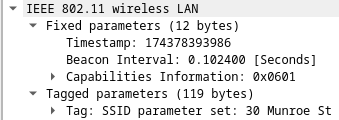
\includegraphics[width=\textwidth]{images/tramaMunEx5.png}  
    \caption{Trama 1995}
    \label{fig:tramaMunEx5}
\end{figure}
Nas figuras \ref{fig:tramaLinkEx5} e \ref{fig:tramaMunEx5} estão representadas duas
tramas consecutivas correspondentes aos APs de SSIDs linkysys\_SES\_24086 e 30
Munroe St, respetivamente. Reparando no campo Beacon Interval reparamos que o
intervalo de tempo entre a transmissão de tramas é 0.102400 segundos nos dois APs.
Na prática nem sempre a periodicidade é verificada graças a neste tipo de
ligações existir uma maior probabilidade de haver interferências externas e
atenuação do sinal.

\section{Exercício 6}
\textbf{Qual é (em notação hexadecimal) o endereço MAC de origem da trama beacon
de 30 Munroe ST? Para detalhes sobre a estrutura das tramas 802.11, veja a
secção 7 da norma IEEE 802.11 citada no início.}

\begin{figure}[H]
    \centering 
    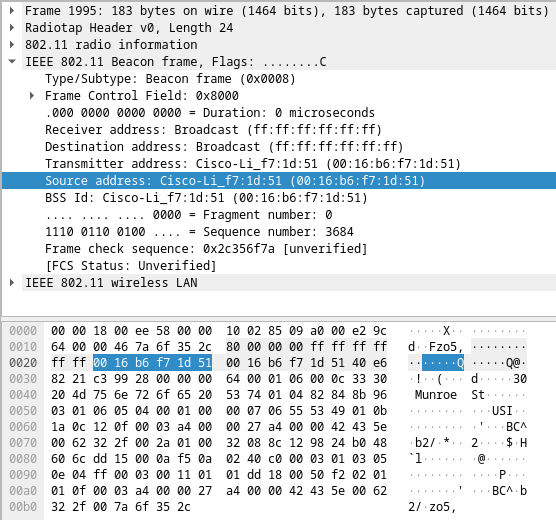
\includegraphics[width=\textwidth]{images/tramaEx6.png}  
    \caption{Trama 1995}
    \label{fig:tramaEx6}
\end{figure}
Observando o campo Source Address da figura \ref{fig:tramaEx6} vemos que o
endereço MAC de origem é 00:16:b6:f7:1d:51.

\section{Exercício 7}
\textbf{Qual é (em notação hexadecimal) o endereço MAC de destino na trama de 30
Munroe ST??}\\
Observando o campo Destination Address da figura anterior vemos que o endereço
MAC de destino é ff:ff:ff:ff:ff:ff.

\section{Exercício 8}
\textbf{Qual é (em notação hexadecimal) o MAC BSS ID da trama beacon de 20
Munroe ST?}\\
Observando o campo BSS Id da figura anterior vemos que o o MAC BSS ID é
00:16:b6:f7:1d:51.

\section{Exercício 9}
\textbf{As tramas beacon do AP 30 Munroe St anunciam que o AP suporta quatro
data rates e oito extended supported rates adicionais. Quais são?}

\begin{figure}[H]
    \centering 
    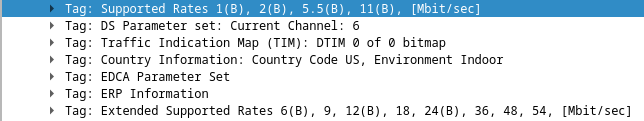
\includegraphics[width=\textwidth]{images/supportedRatesEx9.png}  
    \caption{Data e Supported Rates}
    \label{fig:supportedRatesEx9}
\end{figure}
Observando a figura \ref{fig:supportedRatesEx9}, reparamos que as tramas do AP
30 Munroe St suportam débitos de base de 1 até 11 MBs e extended supported rates de
6 a 54 MBs.

\section{Exercício 10}
\textbf{Selecione uma trama beacon (e.g., a trama 1YXX com Y=turno e XX=grupo,
e.g., 1101). Esta trama pertence a que tipo de tramas 802.11? Indique o
valor dos seus identificadores de tipo e de subtipo. Em que parte concreta
do cabeçalho da trama estão especificados (ver anexo)?}

\begin{figure}[H]
    \centering 
    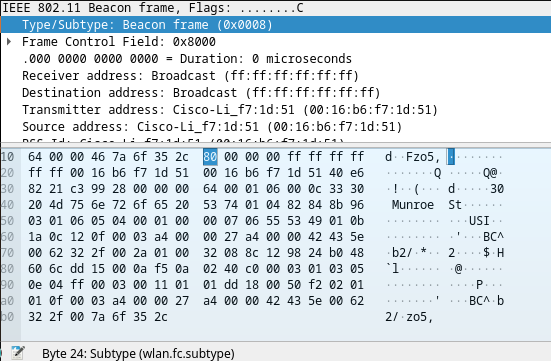
\includegraphics[width=\textwidth]{images/tipoEx10.png}  
    \caption{Tipo da trama 1995}
    \label{fig:tipoEx10}
\end{figure}
Analisando a figura \ref{fig:tipoEx10}, reparamos que esta trama corresponde a
uma trama de gestão (Management type). O identificador é do tipo 0 (0x00) e o
subtipo 8 (0x1000). No cabeçalho esta informação encontra-se no byte 24.

\section{Exercício 11}
\textbf{Verifique se está a ser usado o método de deteção de erros CRC e se
todas as tramas beacon são recebidas corretamente. Justifique o uso de
mecanismos de deteção de erros neste tipo de redes locais.}

\begin{figure}[H]
    \centering 
    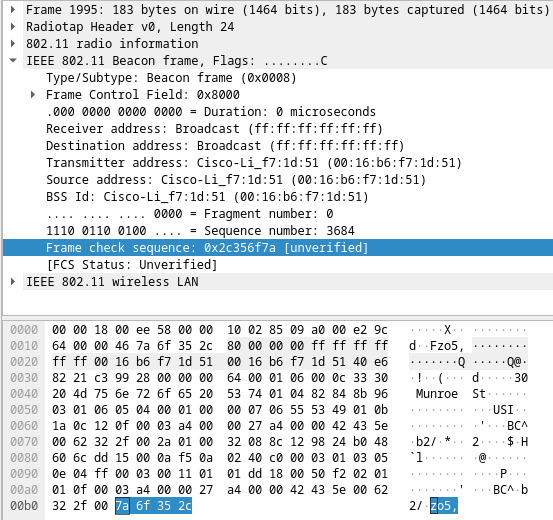
\includegraphics[width=\textwidth]{images/erroEx11.png}  
    \caption{Frame check sequence}
    \label{fig:erroEx11}
\end{figure}
Primeiramente começamos por usar um filtro, wlan.fc.type\_subtype==0x0008 \&\&
wlan.fcs.status==bad, de modo a verificar se existiam tramas com esse estado
"bad". No entanto, nenhuma trama foi encontrada. Seguidamente analisamos algumas
tramas manualmente e reparamos (tal como mostrado na figura \ref{fig:erroEx11})
que todas as tramas tinham "unverified" no campo Fram Check Sequence. Logo, o
método de deteção de erros CRC não está a ser usado.

\section{Exercício 12}
\textbf{Identifique e registe todos os endereços MAC usados nas tramas beacon
enviadas pelos APs. Recorde que o endereçamento está definido no cabeçalho
das tramas 802.11 podendo ser utilizados até quatro endereços com diferente
semântica. Para uma descrição detalhada da estrutura da trama 802.11,
consulte o anexo ao enunciado.}

\begin{figure}[H]
    \centering 
    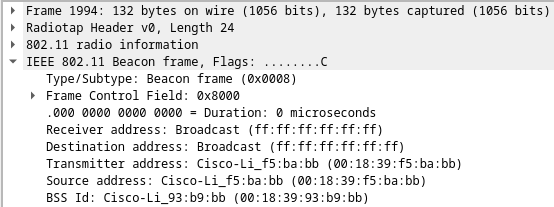
\includegraphics[width=\textwidth]{images/trama1994Ex12.png}  
    \caption{Trama 1994}
    \label{fig:trama1994Ex12}
\end{figure}

\begin{figure}[H]
    \centering
    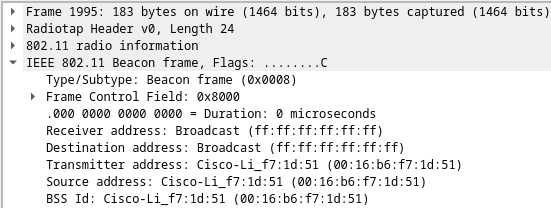
\includegraphics[width=\textwidth]{images/trama1995Ex12.png}  
    \caption{Trama 1995}
    \label{fig:trama1995Ex12}
\end{figure}
Nas tramas beacon enviadas pelos APs estão presentes quatro endereços: Receiver
Address, Destination Address, Transmiter Address e Source Address. Analisando
as figuras \ref{fig:trama1994Ex12} e \ref{fig:trama1995Ex12} vemos que em todas as
tramas o Receiver e o Destination address tem o valor ff:ff:ff:ff:ff:ff
(Broadcast). Relativamente aos outros dois endereços, para o AP da trama 1994 
o Transmitter e Source Address é Cisco\_Li\_f5:ba:bb (00:18:39:f5:ba:bb) e para
o AP da trama 1995 é Cisco\_Li\_f7:1d:51 (00:16:b6:f7:1d:51).

\section{Exercício 13}
\textbf{Estabeleça um filtro Wireshark apropriado que lhe permita visualizar
todas as tramas probing request e probing response, simultaneamente.}

\begin{figure}[H]
    \centering 
    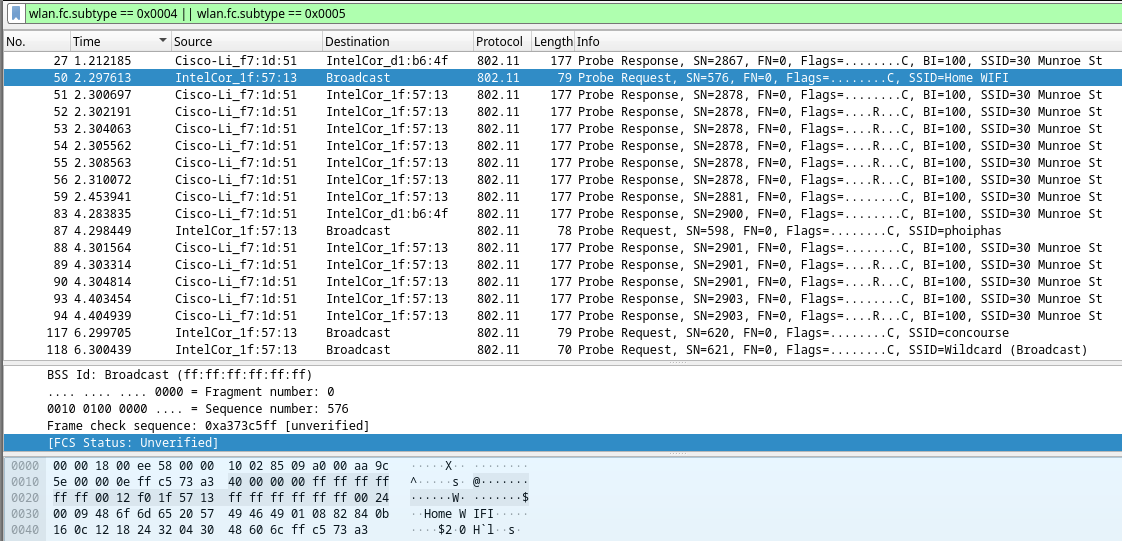
\includegraphics[width=\textwidth]{images/filtroEx13.png}  
    \caption{Filtro Wireshark}
    \label{fig:filtroEx3}
\end{figure}
Como é possível observar pela figura \ref{filtroEx13}, o filtro "wlan.fc.subtype 
== 0x0004 || wlan.fc.subtype == 0x0005" mostra as tramas do tipo Probing Request
e Response, pois estas tem o valor de subtipo 4 e 5, respetivamente.

\section{Exercício 14}
\textbf{Quais são os endereços MAC BSS ID de destino e origem nestas tramas?
Qual o objetivo deste tipo de tramas?}\\
Observando a figura \ref{fig:filtroEx13} podemos ver que a trama de subtipo Probing 
Request tem como BSS ID de origem IntelCor\_1f:57:13 e destino Broadcast. Isto 
significa que foi feito um pedido para todos os equipamentos da rede de modo a encontrar
um AP. A trama seguinte de subtipo Probing Response é a resposta à anterior, em que o BSS
ID de origem é Cisco\_Li\_f7:1d:51 e de destino IntelCor\_1f:57:13.

\section{Exercício 15}
\textbf{Identifique um probing request para o qual tenha havido um probing
response. Face ao endereçamento usado, indique a que sistemas são
endereçadas estas tramas e explique qual o propósito das mesmas?}

\begin{figure}[H]
    \centering 
    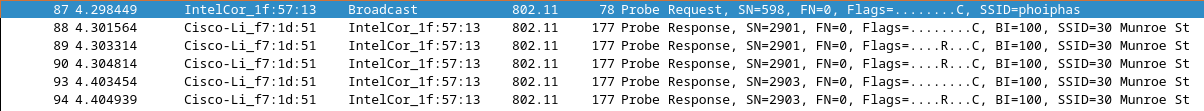
\includegraphics[width=\textwidth]{images/probEx15.png}  
    \caption{Prob Request e Prob Response}
    \label{fig:probEx15}
\end{figure}
Observando a figura \ref{fig:probEx15} verificamos que a trama 87 é um Probing Request e a 
trama 88 é o Probing Response correspondente. Relativamente aos endereços, na primeira 
trama esse corresponde ao STA (IntelCor\_1f:57:13), que emite para todos os equipamentos da
rede de forma a encontrar um AP e na segunda esse corresponde ao AP (Cisco\_Li\_f7:1d:51) que
por sua vez enviou uma resposta.

\chapter{6. Processo de Associação}
\section{Exercício 16}
\textbf{Quais as duas ações realizadas (i.e., tramas enviadas) pelo host no
trace imediatamente após t=49 para terminar a associação com o AP 30 Munroe
St que estava ativa quando o trace teve inicio? (Pista: uma é na camada IP e
outra na camada de ligação 802.11). Observando a especificação 802.11, seria
de esperar outra trama, mas que não aparece?}

\begin{figure}[H]
    \centering 
    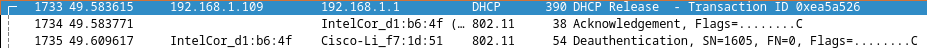
\includegraphics[width=\textwidth]{images/acoesEx16.png}  
    \caption{Ações realizadas pelo host}
    \label{fig:acoesEx16}
\end{figure}
Como se pode ver na figura \ref{fig:acoesEx16}, as ações realizadas pelo host
são as tramas 1733 e 1735, em que na primeira liberta a ligação e na segunda 
termina a autenticação.

\section{Exercício 17}
\textbf{Examine o trace e procure tramas de authentication enviadas do host para
um AP e vice-versa. Quantas mensagens de authentication foram enviadas do
host para o AP linkysys\_ses\_24086 (que tem o endereço MAC
Cisco\_Li\_f5:ba:bb) aproximadamente ao t=49?}

\begin{figure}[H]
    \centering 
    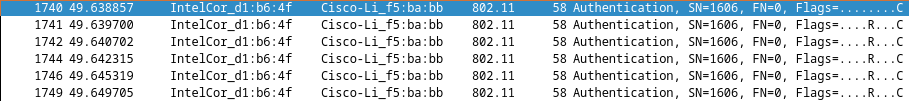
\includegraphics[width=\textwidth]{images/authenticationEx17.png}  
    \caption{Tramas authentication enviadas}
    \label{fig:authenticationEx17}
\end{figure}
Analisando a figura \ref{fig:authenticationEx17} reparamos que foram enviadas
6 tramas de autenticação.


\section{Exercício 18}
\textbf{Qual o tipo de autenticação pretendida pelo host, aberta ou usando uma
chave?}\\

\begin{figure}[H]
    \centering 
    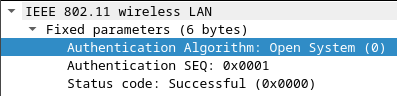
\includegraphics[width=\textwidth]{images/authenticationEx18.png}  
    \caption{Authentication Agorithm}
    \label{fig:authenticationEx18}
\end{figure}
Observando o campo "Authentication Algorithm" da figura \ref{fig:authenticationEx18}
podemos ver que se trata de uma autenticação aberta.

\section{Exercício 19}
\textbf{Observa-se a resposta de authentication do AP linksys\_ses\_24086 AP no
trace?}\\

\begin{figure}[H]
    \centering 
    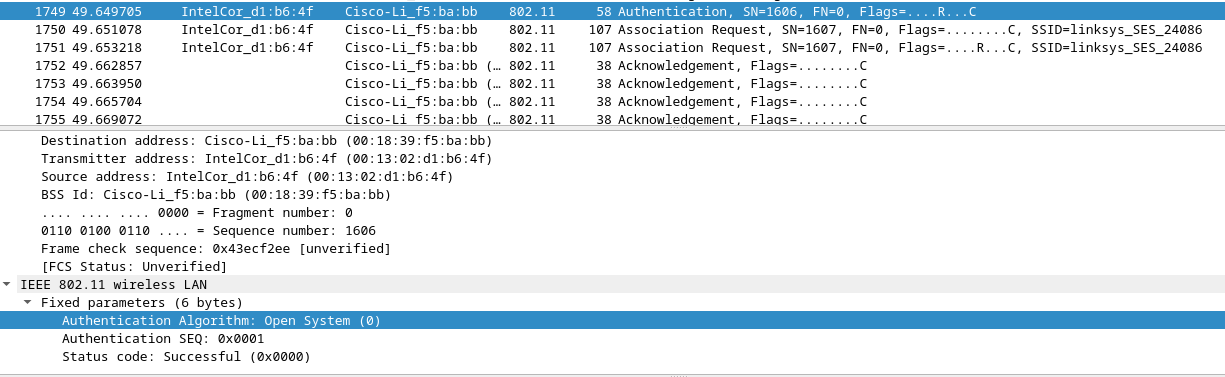
\includegraphics[width=\textwidth]{images/tramasEx19.png}  
    \caption{Tramas após a autenticação}
    \label{fig:tramasEx19}
\end{figure}
Analisando as tramas seguidas da 1749 na figura \ref{fig:tramasEx19} reparamos 
que não existe qualquer trama que indique uma resposta do AP.

\section{Exercício 20}
\textbf{Vamos agora considerar o que acontece quando o host desiste de se
associar ao AP linksys\_ses\_24086 AP e se tenta associar ao AP 30 Munroe
St. Procure tramas authentication enviadas pelo host para e do AP e
vice-versa. Em que tempo aparece um trama authentication do host para o AP
30 Munroe St. e quando aparece a resposta authentication do AP para o
host?}\\

\begin{figure}[H]
    \centering 
    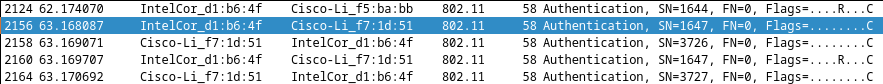
\includegraphics[width=\textwidth]{images/respostaEx20.png}  
    \caption{Tramas authentication}
    \label{fig:respostaEx20}
\end{figure}
Podemos ver na figura \ref{fig:respostaEx20} que a trama de authentication do
host para o AP (2156) aparece no tempo 63.168087 e a trama de autenticação do 
AP para o host (2158) aparece no tempo 63.169071. 

\section{Exercício 21}
\textbf{Um associate request do host para o AP e uma trama de associate response
correspondente do AP para o host são usados para que o host seja associado a
um AP. Quando aparece o associate request do host para o AP 30 Munroe St?
Quando é enviado o correspondente associate reply?}\\

\begin{figure}[H]
    \centering 
    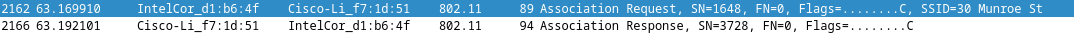
\includegraphics[width=\textwidth]{images/associationEx21.png}  
    \caption{Associate Request e Response}
    \label{fig:associationEx21}
\end{figure}
Observando a figura \ref{fig:associationEx21}, o association request foi feito 
no tempo 63.169910 (trama 2162) e a resposta foi feita no tempo 63.192101 
(trama 2166).

\section{Exercício 22}
\textbf{Que taxas de transmissão o host está disposto a usar? E o AP?}\\

\begin{figure}[H]
    \centering 
    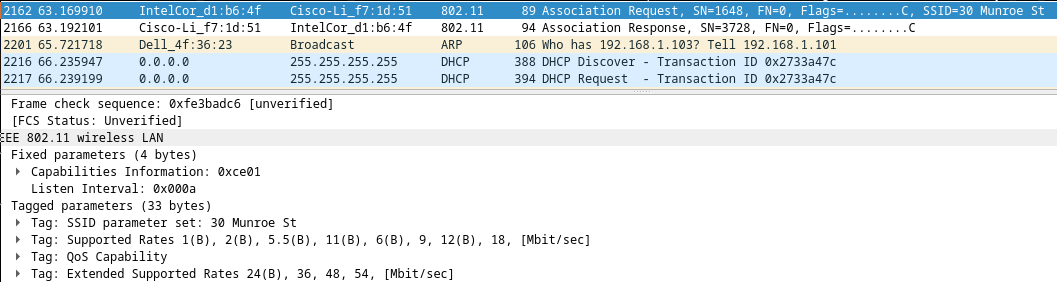
\includegraphics[width=\textwidth]{images/hostEx22.png}  
    \caption{Taxas de transmissão do Host}
    \label{fig:hostEx22}
\end{figure}

\begin{figure}[H]
    \centering 
    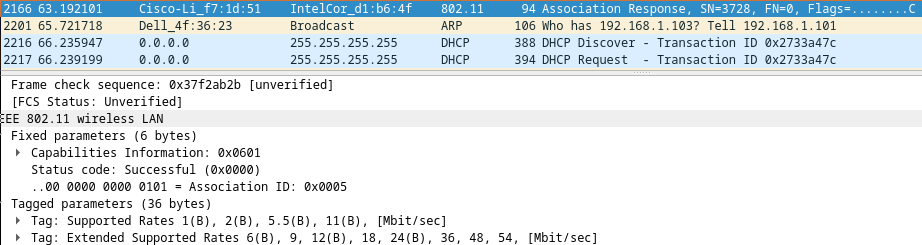
\includegraphics[width=\textwidth]{images/apEx22.png}  
    \caption{Taxas de transmissão do AP}
    \label{fig:apEx22}
\end{figure}
Analisando as figuras \ref{fig:hostEx22} e \ref{fig:apEx22}, conseguimos ver que
as taxas de transmissão que o host e o AP estão dispostos a usar chegam a 54 Mbit/sec.

\section{Exercício 23}
\textbf{Identifique uma sequência de tramas que corresponda a um processo de
associação completo entre a STA e o AP, incluindo a fase de autenticação.}\\
Para facilitar a procura de um processo de associação completo, começamos por aplicar
um filtro (figura \ref{fig:filterEx23}). Seguidamente, selecionamos as tramas 2162 e 2166.

\begin{figure}[H]
    \centering 
    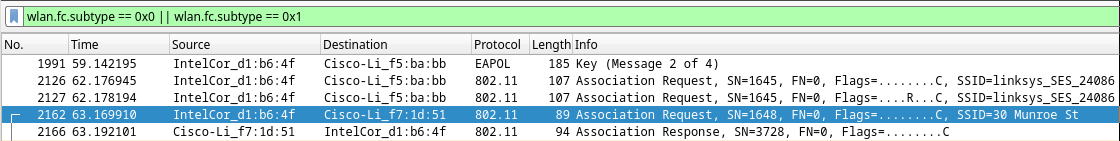
\includegraphics[width=\textwidth]{images/filterEx23.png}  
    \caption{Taxas de transmissão do AP}
    \label{fig:filterEx23}
\end{figure}
Logo após, removemos o filtro e identificamos todas as tramas correspondentes ao processo 
de autenticação (tramas 2156 a 2167). A fase de autenticação começa com três
tramas de autenticação (trama 2156, 2158 e 2160) e as três de confirmação
(tramas 2157, 2159 e 2161). Na trama 2162 acontece um Authentication Request,
seguindo de uma autenticação (trama 2164) e duas confirmações (tramas 2163 e
2165). Termina com um Association response (trama 2166) seguido da sua
confirmação (trama 2167).

\begin{figure}[H]
    \centering 
    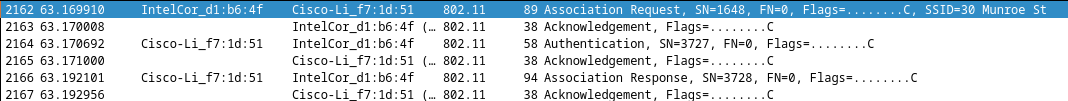
\includegraphics[width=\textwidth]{images/nofilterEx23.png}  
    \caption{Taxas de transmissão do AP}
    \label{fig:nofilterEx23}
\end{figure}

\section{Exercício 24}
\textbf{Efetue um diagrama que ilustre a sequência de todas as tramas trocadas
no processo de associação, incluindo a fase de autenticação}\\
No diagrama seguinte está presente a sequência de todas as tramas trocadas no
progresso de associação, incluindo a fase de autenticação.

\begin{figure}[H]
    \centering 
    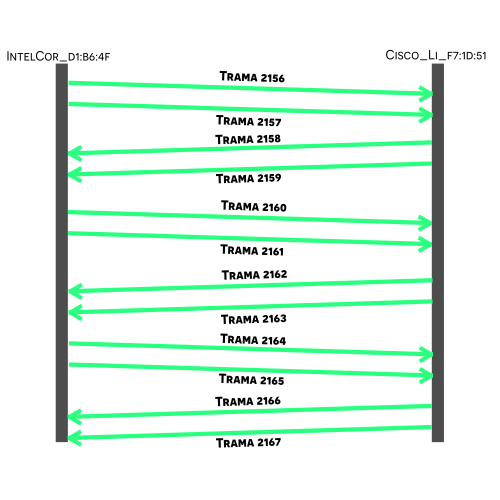
\includegraphics[width=\textwidth]{images/diagramaEx24.png}  
    \caption{Diagrama}
    \label{fig:diagramaEx24}
\end{figure}

\chapter{7. Transferência de Dados}

\section{Exercício 25}
\textbf{Encontre a trama 802.11 que contém o segmento SYN TCP para a primeira
sessão TCP (download alice.txt). Quais são os três campos dos endereços MAC
na trama 802.11?}\\

\begin{figure}[H]
    \centering 
    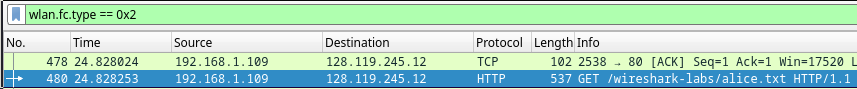
\includegraphics[width=\textwidth]{images/tramaEx25.png}  
    \caption{Trama com o segmento SYN TCP}
    \label{fig:tramaEx25}
\end{figure}
Analisando a figura \ref{fig:tramaEx25}, reparamos que o Destination address é
Cisco\_Li\_f4:eb:a8 (00:16:b6:f4:eb:a8), Source Address é IntelCor\_d1:b6:4f 
(00:13:02:d1:b6:4f) e BSS Id é Cisco\_Li\_f7:1d:51 (00:16:b6:f7:1d:51).

\section{Exercício 26}
\textbf{Qual o endereço MAC nesta trama que corresponde ao host (em notação
hexadecimal)? Qual o do AP? Qual o do router do primeiro salto? Qual o
endereço IP do host que está a enviar este segmento TCP? Qual o endereço IP
de destino?}\\
O endereço do Source Address corresponde ao host, o Receiver Address ao AP e o 
Destination Address ao router do primeiro salto. O endereço de IP correspondente
ao host que está a enviar este segmento é 192.168.1.209 e o IP de destino é
128.119.245.12.

\section{Exercício 27}
\textbf{Este endereço IP de destino corresponde ao host, AP, router do primeiro
salto, ou outro equipamento de rede? Justifique.}\\
O endereço de IP do destino corresponde a router do primeiro salto.

\section{Exercício 28}
\textbf{Encontre agora a trama 802.11 que contém o segmento SYNACK para esta
sessão TCP. Quais são os três campos dos endereços MAC na trama 802.11?}\\

\begin{figure}[H]
    \centering 
    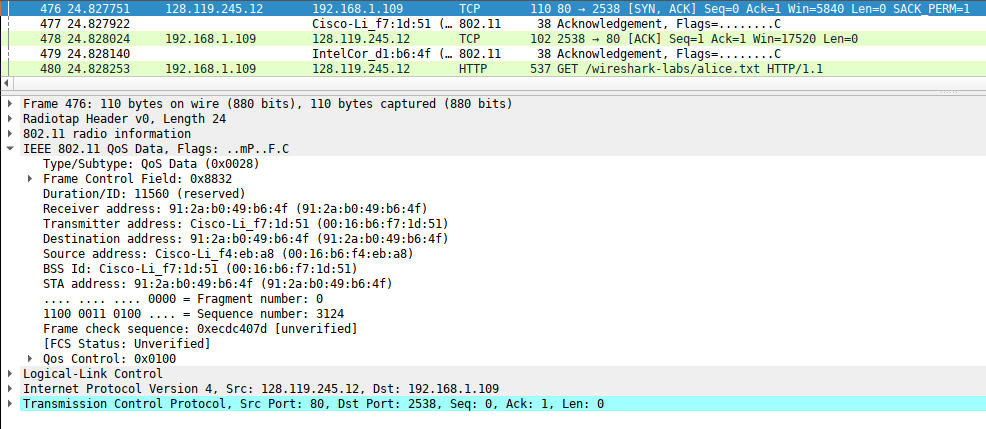
\includegraphics[width=\textwidth]{images/tramaEx28.png}  
    \caption{Trama com o segmento SYNACK}
    \label{fig:tramaEx28}
\end{figure}
Analisando a figura \ref{fig:tramaEx28}, reparamos que o Destination address é
91:2a:b0:49:b6:4f, Source Address é Cisco\_Li\_f4:eb:a8 
(00:16:b6:f4:eb:a8) e BSS Id é Cisco\_Li\_f7:1d:51 (00:16:b6:f4:eb:a8).

\section{Exercício 29}
\textbf{Qual o endereço MAC nesta trama que corresponde ao host? Qual o do AP?
Qual o do router do primeiro salto?}\\
O endereço MAC correspondente ao host é Cisco\_Li\_f7:1d:51 (00:16:b6:f4:eb:a8)
e ao AP e router de primeiro salto é 91:2a:b0:49:b6:4f.

\section{Exercício 30}
\textbf{O endereço MAC de origem na trama corresponde ao endereço IP do
dispositivo que enviou o segmento TCP encapsulado neste datagrama?
Justifique.}\\
Analisando as figuras \ref{fig:tramaEx25} e \ref{tramaEx28} reparamos que o
Transmitter address e o Source Address não são iguais, logo não
corresponde.


\chapter{Conclusão}
Neste trabalho prático tivemos a oportunidade de explorar vários aspetos do
protocolo IEEE 802.11 analisando a captura que nos foi fornecida para realização
deste trabalho.\\
No primeiro capítulo, Acesso Rádio, teve como foco a rede sem fios em si e para
isso analisamos uma ou duas tramas. No capítulo seguinte, o objetivo principal
foi perceber os tipos e subtipos de tramas existentes, analisando
maioritariamente as de gestão. Seguidamente, foi nos pedido para analisar e
perceber como é feita a autenticação e associação nas redes. Por último, tivemos
que compreender como é feita a transferência de dados tendo que analisar o
download de um ficheiro de texto.


\end{document}
